
%(BEGIN_QUESTION)
% Copyright 2008, Tony R. Kuphaldt, released under the Creative Commons Attribution License (v 1.0)
% This means you may do almost anything with this work of mine, so long as you give me proper credit

En kloranalysator måler klorkonsentrasjonen i avløpsvann for å avgjøre om det finnes nok oppløst klor til å desinfisere vannet før utslipp til en naturlig resipient som elv eller bukt:

$$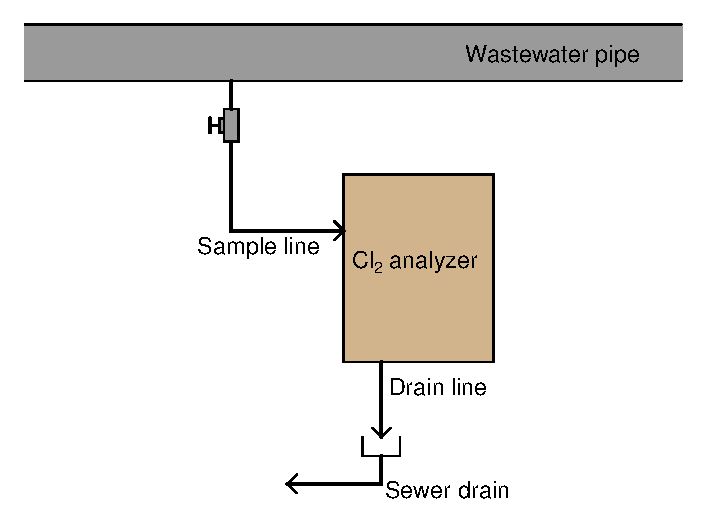
\includegraphics[width=15.5cm]{i00679x01.eps}$$

Det finnes imidlertid et problem i dette systemet: ventiler og slanger inne i kloranalysatoren sprekker fordi prøvetrykket er for høyt. Analysatoren er designet for maksimalt 1 PSI prøvevanntrykk, mens røret er trykksatt til 10 PSI.

\filbreak

En instrumenttekniker finner en løsning. Løsningen innebærer å installere et åpent "standpipe" der vann fra hovedrøret går inn før det strømmer videre til analysatoren:

$$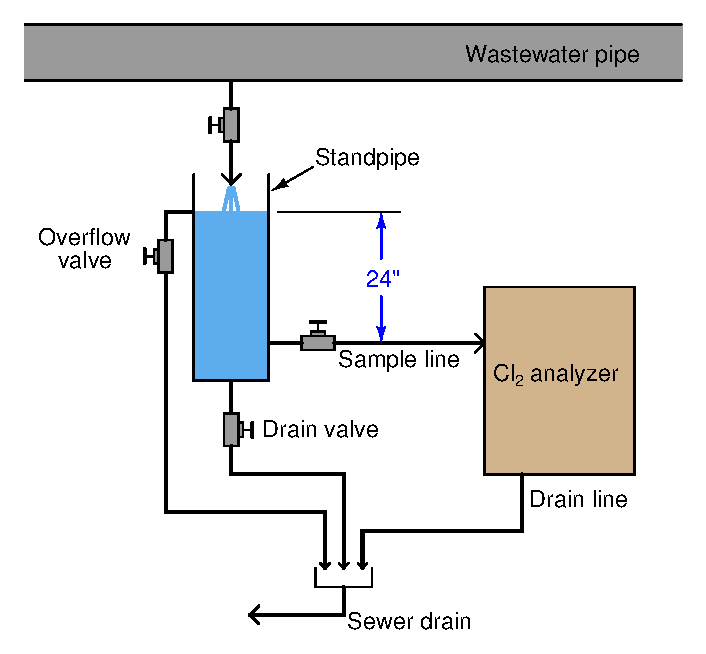
\includegraphics[width=15.5cm]{i00679x02.eps}$$

Beskriv hvordan denne løsningen unngår overtrykksproblemet.

\underbar{file i00679no}
%(END_QUESTION)





%(BEGIN_ANSWER)

Med standpipe installert går avløpsvannet til analysatoren kun ved tyngdekraft (hydrostatisk trykk). Trykket i hovedrøret er da helt isolert fra analysatoren.

%(END_ANSWER)





%(BEGIN_NOTES)

Dette problemet ble møtt og løst av en tidligere student (Bryce VanWerven) på arbeidsplassen hans i et kommunalt avløpsrenseanlegg. Standpipe-løsningen er hans idé, ikke min.

%INDEX% Måling, analytisk: klor i vann
%INDEX% Fysikk, statiske væsker: hydrostatisk trykk

%(END_NOTES)
